% Important: If latex complains about unicode characters,
% please use "\usepackage[utf8x]{inputenc}" in your preamble
% You can change the size of the picture by putting it into the construct:
% 1) \resizebox{10cm}{!}{"below picture"} to scale horizontally to 10 cm
% 2) \resizebox{!}{15cm}{"below picture"} to scale vertically to 15 cm
% 3) \resizebox{10cm}{15cm}{"below picture"} a combination of above two
% It is not recomended to use the scale option of the tikzpicture environment.
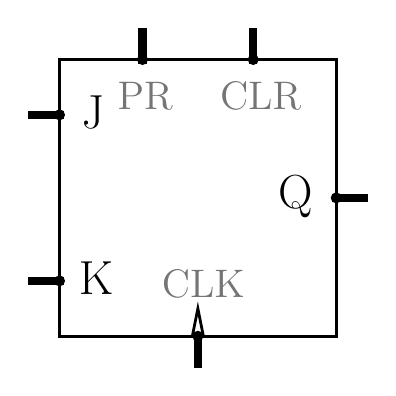
\begin{tikzpicture}[x=1pt,y=-1pt,line cap=rect]
\def\logisimfontA#1{\fontfamily{cmr}{#1}} % Replaced by logisim, original font was "SansSerif"
\def\logisimfontB#1{\fontfamily{Ubuntu}{#1}}
\definecolor{custcol_0_0_0}{RGB}{0, 0, 0}
\definecolor{custcol_75_75_75}{RGB}{117, 117, 117}
\definecolor{custcol_ff_ff_ff}{RGB}{255, 255, 255}
\draw [line width=3.0pt, custcol_0_0_0 ]  (65.0,115.0) -- (65.0,125.0) ;
\draw [line width=3.0pt, custcol_0_0_0 ]  (5.0,95.0) -- (15.0,95.0) ;
\draw [line width=3.0pt, custcol_0_0_0 ]  (115.0,65.0) -- (125.0,65.0) ;
\draw [line width=3.0pt, custcol_0_0_0 ]  (5.0,35.0) -- (15.0,35.0) ;
\draw [line width=3.0pt, custcol_0_0_0 ]  (45.0,5.0) -- (45.0,15.0) ;
\draw [line width=3.0pt, custcol_0_0_0 ]  (85.0,5.0) -- (85.0,15.0) ;
\draw [line width=1.0pt, custcol_0_0_0 ]  (15.0,15.0) -- (114.0,15.0) ;
\draw [line width=1.0pt, custcol_0_0_0 ]  (115.0,15.0) -- (115.0,114.0) ;
\draw [line width=1.0pt, custcol_0_0_0 ]  (115.0,115.0) -- (16.0,115.0) ;
\draw [line width=1.0pt, custcol_0_0_0 ]  (15.0,115.0) -- (15.0,16.0) ;
\draw [line width=1.0pt, custcol_0_0_0 ]  (65.0,105.0) -- (63.0,115.0) -- (67.0,115.0) -- cycle;
\logisimfontB{\fontsize{16pt}{16pt}\fontseries{bx}\selectfont\node[inner sep=0, outer sep=0, custcol_0_0_0, anchor=base west] at  (23.0,40.0)  {J};}
\logisimfontB{\fontsize{16pt}{16pt}\fontseries{bx}\selectfont\node[inner sep=0, outer sep=0, custcol_0_0_0, anchor=base west] at  (22.0,100.0)  {K};}
\logisimfontB{\fontsize{16pt}{16pt}\fontseries{bx}\selectfont\node[inner sep=0, outer sep=0, custcol_0_0_0, anchor=base west] at  (94.0,69.0)  {Q};}
\logisimfontB{\fontsize{14pt}{14pt}\fontseries{bx}\selectfont\node[inner sep=0, outer sep=0, custcol_75_75_75, anchor=base west] at  (36.0,33.0)  {PR};}
\logisimfontB{\fontsize{14pt}{14pt}\fontseries{bx}\selectfont\node[inner sep=0, outer sep=0, custcol_75_75_75, anchor=base west] at  (73.0,33.0)  {CLR};}
\logisimfontB{\fontsize{14pt}{14pt}\fontseries{bx}\selectfont\node[inner sep=0, outer sep=0, custcol_75_75_75, anchor=base west] at  (52.0,101.0)  {CLK};}
\fill [line width=1.0pt, custcol_0_0_0]  (15.0,35.0) ellipse (2.0 and 2.0 );
\fill [line width=1.0pt, custcol_0_0_0]  (15.0,95.0) ellipse (2.0 and 2.0 );
\fill [line width=1.0pt, custcol_0_0_0]  (45.0,15.0) ellipse (2.0 and 2.0 );
\fill [line width=1.0pt, custcol_0_0_0]  (65.0,115.0) ellipse (2.0 and 2.0 );
\fill [line width=1.0pt, custcol_0_0_0]  (85.0,15.0) ellipse (2.0 and 2.0 );
\fill [line width=1.0pt, custcol_0_0_0]  (115.0,65.0) ellipse (2.0 and 2.0 );
\end{tikzpicture}

